%This is a test file to determine the layout of the Owl Datasheet
\documentclass{article}
\pagestyle{myheadings}
\markright{BBa\_K1179002}
\usepackage[xcolor]{mdframed} %Top header has banner!
\usepackage{hyphenat} %Column titles are not to have hyphenation
\usepackage{seqsplit} %Manages long DNA sequence line breaks
\usepackage{ccaption} %Formatting table titles
\usepackage[margin=1in]{geometry} %Setting document margins
\usepackage{graphicx} %Using images
\usepackage{array} %Formatting table size and behavior
\begin{document}
\renewcommand{\topfraction}{0.99} %Helps with keeping whitespace to a minimum
\renewcommand{\textfraction}{0.99}
\renewcommand{\floatpagefraction}{0.99}
\begin{table}[htbp]
\setlength{\belowcaptionskip}{4pt}
\setlength{\extrarowheight}{8pt}
\begin{mdframed}[backgroundcolor=gray!32,topline=false,rightline=false,leftline=false,bottomline=false] \legend{\Huge \underline{BBa\_K1179002}} \end{mdframed} \hfill \break
\begin{tabular}{m{1.2in}m{4.98in}}
\large \textbf{\nohyphens{Part Summary}} & This part encodes for the constitutive expression of a Cas9-VP16 fusion protein. The Cas9 has been mutated in such a way as to remove its nuclease activity while retaining its ability to selectively bind DNA mediated by an appropriate guide RNA (gRNA). The Cas9-VP16 complexes with an expressed gRNA and together target a DNA sequence as defined by the gRNA. Once the Cas9-VP16 is bound, the VP16 domain can activate a downstream inducible promoter like minimal CMV.\\
\large \textbf{\nohyphens{Part Type}} & Composite Part\\
\large \textbf{\nohyphens{Pigeon Image}} & \hfill \break 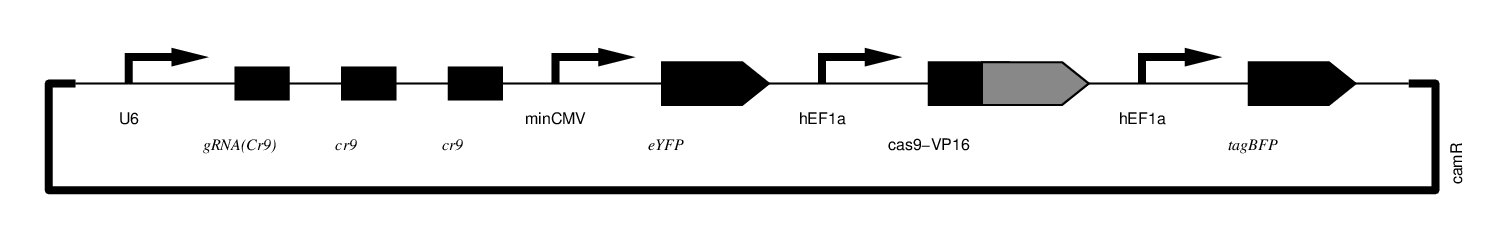
\includegraphics[width=10cm,height=10cm,keepaspectratio]{/Users/Zach/Documents/Owl/igem-datasheet/Datasheet_Generator/src/main/webapp/tmp/1439914929945BBa_K1179002_pigeon.png} \\ 
\large \textbf{\nohyphens{Plasmid Map}} & \hfill \break 
\includegraphics[width=10cm,height=10cm,keepaspectratio]{/Users/Zach/Documents/Owl/igem-datasheet/Datasheet_Generator/src/main/webapp/tmp/1439914930115BBa_K1179002_plasmid_map.png} \
\end{tabular}
\end{table}
\begin{table}[htbp]
\setlength{\belowcaptionskip}{4pt}
\setlength{\extrarowheight}{8pt}
\begin{mdframed}[backgroundcolor=gray!32,topline=false,rightline=false,leftline=false,bottomline=false] \legend{\LARGE Designer Information}\end{mdframed}
\begin{tabular}{m{1.2in}m{4.98in}}
\large \textbf{\nohyphens{Author(s)}} & Brandon Nadres\\
\large \textbf{\nohyphens{Date}} & September 17, 2013\\
\large \textbf{\nohyphens{Affiliation}} & Massachusetts Institute of Technology, Weiss Lab\\
\large \textbf{\nohyphens{Team}} & \seqsplit{iGEM13\_MIT}\\
\large \textbf{\nohyphens{Contact}} & \seqsplit{igem-2013@mit.edu}
\end{tabular}
\end{table}
\begin{table}[htbp]
\setlength{\belowcaptionskip}{4pt}
\setlength{\extrarowheight}{8pt}
\begin{mdframed}[backgroundcolor=gray!32,topline=false,rightline=false,leftline=false,bottomline=false] \legend{\LARGE Design Details}\end{mdframed}
\begin{tabular}{m{1.2in}m{4.98in}}
\large \textbf{\nohyphens{Type}} & \seqsplit{Generator}\\
\large \textbf{\nohyphens{Design Components}} & K779200, J85600, K1179009
\end{tabular}
\end{table}
\begin{table}[htbp]
\setlength{\belowcaptionskip}{4pt}
\setlength{\extrarowheight}{8pt}
\begin{mdframed}[backgroundcolor=gray!32,topline=false,rightline=false,leftline=false,bottomline=false] \legend{\LARGE Assembly Information}\end{mdframed}
\begin{tabular}{m{1.2in}m{4.98in}}
\large \textbf{\nohyphens{Assembly Method(s)}} & Gateway Technologies\\
\large \textbf{\nohyphens{Chassis}} & Homo sapiens\\
\large \textbf{\nohyphens{Strain}} & Human Embryonic Kidney 293\\
\large \textbf{\nohyphens{Scars}} & \seqsplit{y}
\end{tabular}
\end{table}
\begin{table}[htbp]
\setlength{\belowcaptionskip}{4pt}
\setlength{\extrarowheight}{8pt}
\begin{mdframed}[backgroundcolor=gray!32,topline=false,rightline=false,leftline=false,bottomline=false] \legend{\LARGE Flow Cytometry Experiment}\end{mdframed}
\begin{tabular}{m{1.2in}m{4.98in}}
\large \textbf{\nohyphens{Purpose}} & \seqsplit{Characterization}\\
\large \textbf{\nohyphens{Location}} & Massachusetts Institute of Technology\\
\large \textbf{\nohyphens{Transfer Curve Caption}} & On the Y axis, we see the output fluorescence in the FITC channel and our transfection marker fluorescence in the Pacific A channel on the X axis. As expected, we see activation when all components of the system are present, and increasing the amount of transfected guide RNA increased the ability of the Cas9- VP16 to bind to the synthetic upstream Cr9 regulatory sites of the reporter construct. The graph indicates that saturation hasn't occurred, but due to limitations of the Lipofectamine transfection protocol, transfecting the amount needed for saturation would likely be toxic to the cells.\\
\large \textbf{\nohyphens{Transfer Curve Graph}} & \hfill \break 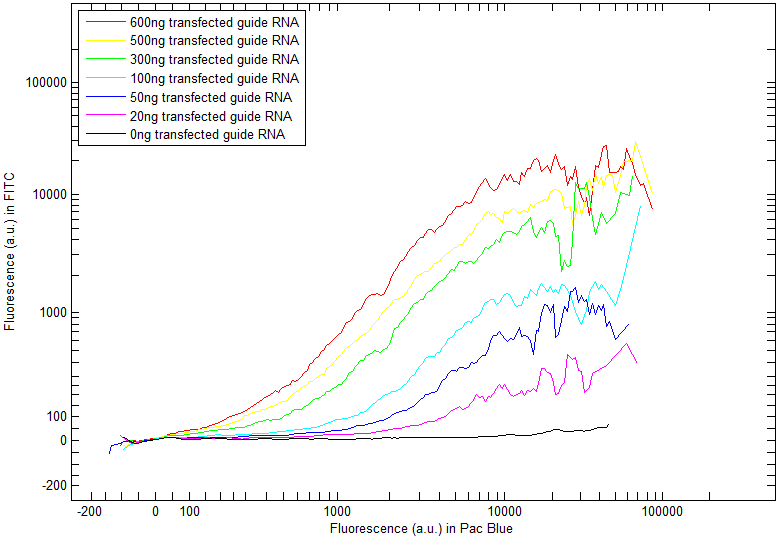
\includegraphics[width=10cm,height=10cm,keepaspectratio]{/Users/Zach/Documents/Owl/igem-datasheet/Datasheet_Generator/src/main/webapp/tmp/1439914930274BBa_K1179002_transfer_curve.png} \
\end{tabular}
\end{table}
\end{document}
